\section{Discussion}
\label{sec:discuss}

In this section we perform further analysis on the clustering output of our
model.  The example below illustrates the advantage of the
instance-based approach:

%% \begin{figure}[ht]
%%   %  \begin{minipage}[c]{\columnwidth}
     \begin{tabular}{ll}
      (1) & $\hdots$ it will also {\bf offer} buyers the option $\hdots$\\
      &{\bf Substitutes:} give, help, attract\\ 
      (2) & The {\bf offer} is being launched $\hdots$\\ 
      &{\bf Substitutes:} campaign, project, scheme\\ 
    \end{tabular}
 %%   \caption{Ambiguous occurrences of the word {\em offer}.}
 %%   \label{fig:typelimitation}
 %%   %\end{minipage} \hfill
 %% \end{figure}

The word {\bf offer} is a {\em verb} in the first sentence and a {\em
  noun} in the second one.  Clustering the word embeddings can not
distinguish the different occurrences of the words
\cite{yatbaz-sert-yuret:2012:EMNLP-CoNLL}.  On the other hand, the
substitutes of {\em offer} in the two sentences can disambiguate the
correct category of the corresponding occurrences.  In our actual
experiments our instance based representation distinguishes the
instances of {\bf offer} as {\em noun} (cluster 26 and 12) and {\em
  verb} (cluster 35).

To illustrate how words are distributed in the induced clusters, we
compare the most frequent clusters of our model in Section~\ref{sec:exp}
with the most frequent gold-tags of PTB in Figure~\ref{plot-hinton}.  
%%We also discuss the effect of coarse gold-tag sets
%%on our model performance.
\begin{figure}[t] \centering
%\vspace*{-10mm}
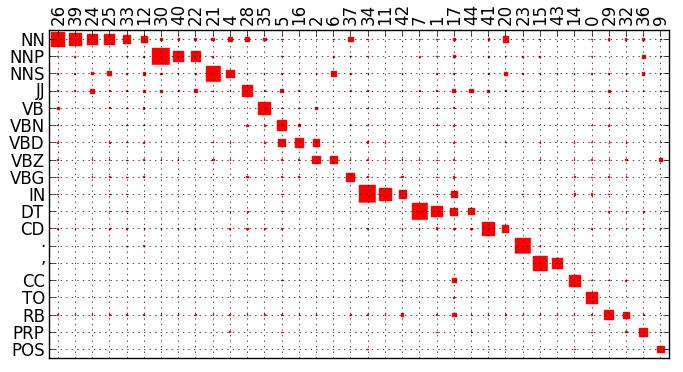
\includegraphics[width=1\columnwidth]{hinton.png}
\caption{Each row corresponds to a gold tag and each column is an
  induced tag in the Hinton diagram above.  The area of each square is
  proportional to the joint probability of the given tag and cluster.
}
  \label{plot-hinton}
\end{figure}

%% Figure~\ref{plot-hinton} is the Hinton diagram of the PTB showing the
%% relationship between gold tags and clusters\footnote{For simplicity only the
%% most frequent gold-tags and clusters are presented.} from the experiment in
%% Section~\ref{sec:instance}. 
The low \vm\ performance of our instance-based model compared to the
state-of-the-art word-based systems on some languages is due to the
completeness part of the \vm\ score.  The Hinton diagram in
Figure~\ref{plot-hinton} shows that large gold-tag groups are split
into several clusters based on the substitutability of words in that
particular cluster (rows of the Hinton diagram).  For example, proper
nouns ({\em NNP}) are split into three major clusters such that titles
like {\em Mr.} or person names are in (40), nationality or country
related words like {\em Japanese} or {U.S} are in (22), and the rest
of the proper nouns in cluster (30).

The gold-tags of PTB, on the other hand, do not always respect whether
words with the same tag are substitutable for one another.
Freudenthal et al.  \shortcite{freudenthal2005resolution} argues, from
the child language acquisition perspective, that the standard
linguistic definition of syntactic groups requires the
substitutability of words in a syntactic category.  Word pairs that
are placed in the same category in the PTB, such as ``Mr.'' and
``Friday'', ``be'' and ``run'', ``not'' and ``gladly'', ``of'' and
``into'' are clearly not generally substitutable.

Another noteworty example of completeness error is that our model splits the
punctuation mark ({\em ,}) class of PTB into the clusters 15 and 43 based on
the different usage patterns.  The majority of the ({\em ,}) instances in
cluster 15 are used in relative clauses, reported speech clauses or
conjunctions while cluster 43 generally consists of ({\em ,}) instances that
are used in non-essential clauses (ex: Time, the largest newsweekly, \ldots). 

%% Another source of completeness error in our model is the split of word
%% instances into several clusters.  For example, all instances of the
%% punctuation mark ({\em ,}) are tagged with same gold-tag in PTB,
%% however our model splits them into cluster 15 and 43 based on usage.

%% To decide whether the completeness or substitutability are better
%% measurement of POS induction, one can perform extrinsic evaluation
%% like parsing or machine translation.

%% Whether gold standard part of speech tags or distributional categories are
%% better suited to applications like parsing or machine translation can be best
%% decided using extrinsic evaluation.  In this study we evaluate our results by
%% comparing them to gold standard part of speech tags and leave the extrinsic
%% evaluations of the induced tags for future work.
%% Here are the some examples from clusters of our model:
%% \begin{itemize}
%%   \item Proper nouns ({\em NNP}) are split into three major clusters such that
%%   titles like {\em Mr.} and person names are in (40), nationality, country or
%%   time related words like {\em Japanese, U.S or Friday} are in (22), and the
%%   rest of the proper nouns in cluster (30).
%% \item Auxiliary verbs (10) and the verb ``say'' (22) have been split
%%   from the general verb clusters (12) and (7).
%% \item Determiners ``the'' (40), ``a'' (15), and capitalized
%%   ``The'', ``A'' (6) have been split into their own clusters.
%% \item Prepositions ``of'' (19), and ``by'', ``at'' (17) have been
%%   split from the general preposition cluster (8).
%% \end{itemize}
%% Nevertheless there are some homogeneity errors as well:
%% \begin{itemize} 
%% \item The adjective cluster (5) also has some noun members probably
%%   due to the difficulty of separating noun-noun compounds from
%%   adjective modification.
%% \item Cluster (6) contains capitalized words that span a number of
%%   categories.
%% \end{itemize}
%% A comparison of morphological structures might be helpful.
%% 
%% Most closed-class items are cleanly separated into their own clusters
%% as seen in the lower right hand corner of the diagram. 
% The sentences in Figure~\ref{fig:typelimitation} illustrates the limitation
% of clustering word embeddings.  

%% The completeness errors become more noticeable on languages with
%% coarse tag-sets thus our models perform worse than the best published
%% models on 6 of MULTEXT-East languages in terms of \vm\ scores while
%% achieving the state-of-the-art \mto\ scores on the same languages as
%% shown on Table~\ref{tab:multiresults}.  On CONLL-X languages the
%% effect of completeness errors is less noticeable since all languages
%% except Czech and Dutch have fine grained tag-sets.

%% The completeness errors are not surprising given that the words that
%% have been split are not generally substitutable with the other members
%% of their gold-tag set category.  Thus it can be argued that metrics
%% that emphasize homogeneity such as \mto\ are more appropriate in this
%% context than metrics that average homogeneity and completeness such as
%% \vm\ as long as the number of clusters is controlled.

%  There are two concerns inherent in all distributional methods: (i)
%  words that are generally substitutable like ``the'' and ``its'' are
%  placed in separate categories ({\sc dt} and {\sc prp\$}) by the gold
%  standard, (ii) words that are generally not substitutable like ``do''
%  and ``put'' are placed in the same category ({\sc vb}).  Freudenthal
%  et al. \shortcite{freudenthal2005resolution} point out that categories
%  with unsubstitutable words fail the standard linguistic definition of
%  a syntactic category and children do not seem to make errors of
%  substituting such words in utterances (e.g. {\em``What do you want?''}
%  vs. {\em *``What put you want?''}).  Whether gold standard part of
%  speech tags or distributional categories are better suited to
%  applications like parsing or machine translation can be best decided
%  using extrinsic evaluation.  In this study we evaluate our results by
%  comparing them to gold standard part of speech tags and leave the
%  extrinsic evaluation of the induced tags for future work.
